\documentclass[letterpaper,twocolumn,superscriptaddress,showkeys]{revtex4}
\usepackage[utf8]{inputenc}
\usepackage{color,dcolumn,graphicx,hyperref}
\hypersetup
{
    colorlinks = true, linkcolor = blue, citecolor = blue, urlcolor = blue,
}

\begin{document}

\title{Open Preprints in Ecology \& Evolution}

\author{Philippe Desjardins-Proulx}
\email[E-mail: ]{philippe.d.proulx@gmail.com}
\affiliation{Theoretical Ecosystem Ecology laboratory, Universit\'e du Qu\'ebec \`a Rimouski, Canada.}
\affiliation{Quebec Center for Biodiversity Science, McGill University, Canada.}
\affiliation{D\'epartement des sciences biologiques, Universit\'e du Qu\'ebec \`a Montr\'eal, Canada.}

\author{Ethan P. White}
\affiliation{Departement of Bology, Utah State University, United-States of America.}

\author{Timoth\'ee Poisot}
\affiliation{Theoretical Ecosystem Ecology laboratory, Universit\'e du Qu\'ebec \`a Rimouski, Canada.}
\affiliation{Quebec Center for Biodiversity Science, McGill University, Canada.}
\affiliation{International Network for Next-Generation Ecology.}

\author{Dominique Gravel}
\affiliation{Theoretical Ecosystem Ecology laboratory, Universit\'e du Qu\'ebec \`a Rimouski, Canada.}
\affiliation{Quebec Center for Biodiversity Science, McGill University, Canada.}

\keywords{Publishing; arXiv; Green Open Access.}

\begin{abstract}

...
 
\end{abstract}

\maketitle

\section{The case for open preprints}

Preprints servers such as arXiv are common in mathematics and physics, but
still a minority of papers in ecology and evolution use them. Preprints
servers allow author to make their manuscripts publicly available before, or
in parallel to, submitting them to journals for traditional peer-review. ...
The idea became popular with arXiv, and many physicists start their day with a
look at the new papers in arXiv \cite{gin11}

We will highlight advantages for both scientists and publishers.

The first and most often discussed advantage is speed \ref{fig:map}.

%% Allows papers to be cited earlier (greater immediacy)

%% @Tim: how can it improve the review process?

The review process as a whole is critically over-loaded, because the number of
active scientists increases, because the pressure to publish increases, and
because of an effect dubbed ``the tragedy of the reviewers commons'' REF.  In
the same times, rejection rates are high in most journals (REF), and when the
not invited to submit a revisions, authors are left with the impression that
they must start the whole process all over again. It's thus no surprize that
different initiatives emerged over the last few years, to decrease the time
spent in review. XXX et coll. (REF) called for the recycling and reuse of
peer-reviews: by attaching previous reviews, and detailed replies, to a new
submission, both the editor and the referees can jauge the work done on the
manuscript, and perhaps evaluate it with less prejudice. In a similar way, the
\emph{Peerage of Science} initiative allows authors to seek anonymous pre-
review by their peers. Some journals (LIST?) now accept to publish papers
which received good evaluations, effectively outsourcing the review process. A
widespread use of preprint servers can achieve the same goal of reducing the
time spent in review. By putting a manuscript out there for open comments and
criticisms, the authors will receive valuable feedback, and can improve the
version which will be submitted. With a rich enough community of scientists
depositing preprints, and commenting on them, the process of an open pre-
review can become widespread, and will overall increase the quality of first
submissions.
% Assuming that the quality of the paper is a good prior of its acceptance probability :-)

\begin{figure}[ht!] \centering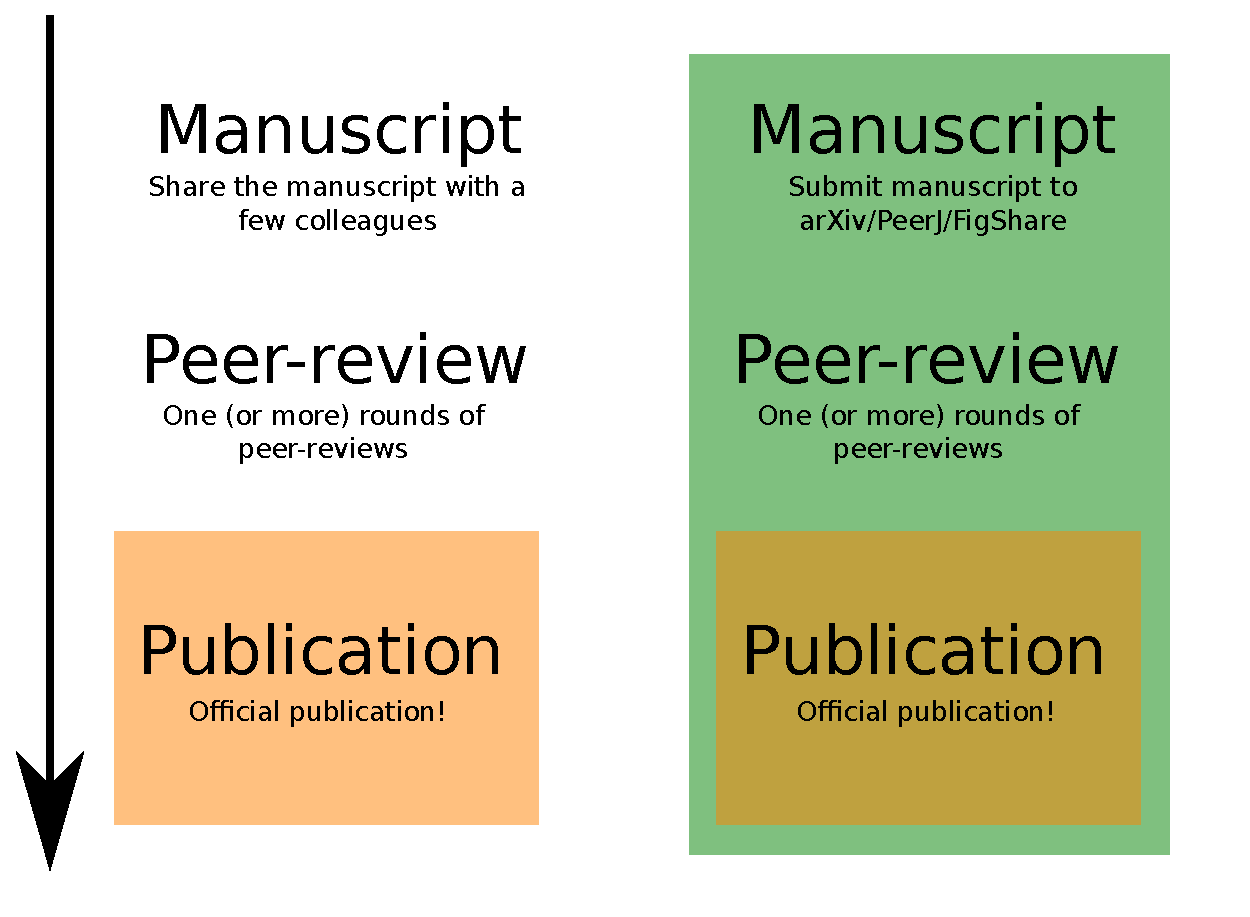
\includegraphics[width=0.50\textwidth]{map.pdf}
\caption { It can take several months, and even a few years, before a submitted
paper is officially published and citable. During this time, few people are
aware of the research that has been done (typically, close colleagues are
given access to the preprints). With public preprint servers, the science is
immediately available and can be openly discussed, analysed, and integrated
into current research. It benefits both science and publishers. Both want the
papers to be well-known and cited, and public preprints make it possible to
integrate research even before publication, greatly improving immediacy.  }
\label{fig:map}
\end{figure}

Preprint servers also establish priority in a fair way. Some manuscript will
spend much more time in the review process. Public preprints server offer a
much fairer way to establish intellectual priority by making the work
available when done, and even if the exact organisation of the manuscript may
change. Surprisingly, there is perception in biology that public preprints
make it easier to steal ideas, as if scientific ideas only took form in
published material.
% TP This needs more development, I'm not sure I get your point
Mathematicians and physicists have embraced arXiv in part
to establish priority in a fair way\cite{cal12}.

Some of the responses to public preprints are surprising since they are,
essentially, the same as exchanging preprints among colleagues.
% TP Well, no. You trust your colleagues, and you trust that they will not give your
%    MS to anyone!
Prepublication reviews by a small network of colleagues is an important part
of the scientific process, which is attested by the fact that nearly all
published papers acknowledge comments by people not listed as co-authors.
Preprints servers simply offer a way to extend this network of colleagues to
the entire scientific community. It ensures that science is not constrained by
small networks of scientists exchanging ideas. Ginsparg made arXiv.org in part
for democratic reasons: he wanted everyone from graduate students in small
universities to Princeton professors to have access to the most recent
scientific \emph{ideas}.
% TP One important point to make: the MS and the idea are different things.
%    We should focus more on the later...
Ginsparg revolutionary idea was simply to use the power of the internet for
preprints, not just for the end product, so the process can be open from A to
Z, instead of being just open at the end of the process.
% TP Since when is the publishing buisness an open process? :-)

\section{Preprints, Ecology \& Evolution}

While the practice is still rare, preprints are becoming more common in
biological sciences, which is experiencing faster growth in arXiv submissions
than any other fields \cite{cal12}. Also, most scientific journals are
preprint-friendly: Nature, PLOS, BMC, PNAS, Science (mostly)
\ref{table:policies}, and all the journals from Elsevier and Springer. Very
recently, the Ecological Society of America recently changed its policy to allow
public preprints (REF). In our field, few scientific publications will not
consider a manuscript submitted to arXiv. Still, many ecology \& evolution journals
adopt a ``by default'' hostile attitude towards preprints, mostly due to the
lack of clear policy of the publishers. As an example, Wiley-Blackwell, which
publishes some of the leading journal in the field, has no official policy on
the subject \ref{table:policies}.

\begin{table*}
    \centering
    \begin{tabular}{|ll|}
    \hline
    Publisher                                   & Policy \\
    \hline
    Springer                            	& Accept \\
    BMC                                 	& Accept \\
    Elsevier                            	& Accept \\
    Nature Publishing Group             	& Accept \\
    Public Library of Science           	& Accept \\
    Royal Society                       	& Accept \\
    National Academy of Science (USA)           & Accept \\
    Science                             	& Accept/Ambiguous \\
    Wiley-Blackwell                       	& No general policy \\
    Ecological Society of America       	& Refuse \\
    British Ecological Society                  & ? \\
    \hline
    \end{tabular}
    \caption{Policies for important publishers in ecology and evolution.}
    \label{table:policies}
\end{table*}

\section{Current offer}

We briefly discuss the main options to submit preprints to open servers:
arXiv.org, Figshare, and the upcoming PeerJ and F1000Research.

\subsection{arXiv}

arXiv (\href{http://arxiv.org/}{http://arxiv.org/}).
arXiv is funded by a network of universities.

...

% @Joel

\subsection{Figshare}

% @PhDP

Figshare (\href{http://figshare.com/}{http://figshare.com/})

All figshare content (article, figures, datasets) have a unique digital object
identifier (DOI) like any journal article.

\subsection{PeerJ}

% @Ethan

\subsection{F1000Research}

% Written from memory: to verify!

F1000Research is not a public preprint server like the previous three servers.
Whereas arXiv, Figshare, and PeerJ offer an option to submit a manuscript
without having it reviewed, papers submitted to F1000Research will eventually be
reviewed. Thus, F1000Research offers a hybrid model with publicly available
manuscripts at time of submission and standard peer-reviews. Manuscripts are
considered ``accepted'' and will only be indexed after two positive referee
response.

\section{Conclusion}

% A short paragraph to conclude.

Responding to the rumour that they refused manuscripts submitted to arXiv,
Nature responded that ``Nature never wishes to stand in the way of communication
between researchers. We seek rather to add value for authors and the community
at large in our peer review, selection and editing'' \cite{nat05}.

\newpage
\bibliography{refs}
\bibliographystyle{plain}

\end{document}

